\documentclass{beamer}
\usetheme{Boadilla}

\usepackage{amsmath}
\usepackage{amsfonts}
\usepackage{hyperref}

\usepackage{amsmath}
\DeclareMathOperator*{\argmax}{arg\,max}
\DeclareMathOperator*{\argmin}{arg\,min}

\title{Can You Trust Your Model’s Uncertainty? Evaluating Predictive Uncertainty Under Dataset Shift}
\author{Dmitry Protasov}
\institute{MIPT, 2023}

\begin{document}

\begin{frame}
    \titlepage
\end{frame}

\begin{frame}
    \tableofcontents
\end{frame}

\section{Motivation}
\begin{frame}{Motivation}
    \begin{block}{}
        Deep Neural Networks (DNNs) are increasingly used in high-stakes applications like medical diagnosis and autonomous driving. In such scenarios, accurately quantifying predictive uncertainty is as important as making point predictions
    \end{block}
\end{frame}

\begin{frame}{Contribution}
    \begin{block}{}
       This study focuses on the challenge of evaluating predictive uncertainty in machine learning models, especially under conditions of dataset shift. A large-scale empirical comparison of Bayesian and non-Bayesian methods for uncertainty estimation is presented. 
    \end{block}
    
\end{frame}

\section{Background}
\begin{frame}{Background}
    \begin{block}{Notation and Problem Setup}
    Let \( x \in \mathbb{R}^d \) represent a set of \( d \)-dimensional features and \( y \in \{1, \ldots, k\} \) denote corresponding labels for \( k \)-class classification. The training dataset \( D \) consists of \( N \) i.i.d. samples \( D = \{(x_n, y_n)\}_{n=1}^N \).
    \end{block}
    \begin{block}{Data Generating Process}
    The true distribution \( p^*(x, y) \), unknown and observed only through the samples \( D \), assumed to be a discrete distribution over \( k \) classes.
    \end{block}

    % We evaluate  the model against OOD inputs sampled from \( q(x, y) \neq p^*(x, y) \). We consider two kinds of shifts
    
    \begin{block}{OOD Inputs}
    Inputs sampled from a distribution \( q(x, y) \) that is different from the training distribution \( p^*(x, y) \), challenging the model's predictive certainty.
    \end{block}
\end{frame}

\begin{frame}{Background}
    We consider two kinds of shifts
    \begin{block}{Covariate Shift}
    Shifts in the distribution of test inputs, potentially leading to a degradation in the accuracy of the model's predictions.
    \end{block}
    \begin{block}{Out-Of-Distribution (OOD) Dataset}
    A test set where the true label is not one of the known \( k \) classes, requiring the model to express higher predictive uncertainty.
    \end{block}
\end{frame}

\begin{frame}{Overview of Uncertainty Estimation Methods}
    \begin{block}{Categories of Methods}
        There are three main categories of machine learning methods for uncertainty estimation and out-of-distribution (OOD) detection:
        \begin{itemize}
            \item Methods which deal with conditional probability \( p(y|x) \) only
            \item Methods modeling the joint distribution \( p(y, x) \)
            \item Methods with an OOD-detection component in addition to \( p(y|x) \)
        \end{itemize}
    \end{block}
    \begin{block}{Note}
        Comparing across these classes of methods is challenging due to differences in modeling assumptions. However, the focus remains on methods that quantify predictive uncertainty.
    \end{block}
\end{frame}

\begin{frame}{Methods}
    \begin{block}{Selected Methods}
    A subset of methods from the probabilistic deep learning literature was selected based on prevalence, scalability, and practical applicability:
    \begin{itemize}
        \item Maximum softmax probability (Vanilla)
        \item Post-hoc calibration by temperature scaling (Temp Scaling)
        \item Monte-Carlo Dropout
        \item Ensembles of networks
        \item Stochastic Variational Bayesian Inference (SVI)
        \item Bayesian inference for the parameters of the last layer only (LL)
        \begin{itemize}
            \item Mean field stochastic variational inference (LL SVI)
            \item Dropout on activations before the last layer (LL Dropout)
        \end{itemize}
    \end{itemize}
    \end{block}
\end{frame}

\begin{frame}{Model Uncertainty Metrics}
    \begin{block}{}
    Metrics to evaluate the quality of model uncertainty under dataset shift
    \begin{itemize}
        \item Negative Log-Likelihood (NLL) --
        can over-emphasize tail probabilities
        \item The Brier Score (BS) -- insensitive to
predicted probabilities associated with in/frequent events:
        \begin{equation}
        BS = \frac{1}{N} \sum_{n=1}^{N} \Big( p(y_n|x_n, \theta) - \delta(y_n - y)\Big)^2
        \end{equation}
        
        \item The Expected Calibration Error (ECE) is:
        \begin{equation}
        ECE = \sum_{s=1}^{S} \frac{|B_s|}{N} |acc(B_s) - conf(B_s)|
        \end{equation}
        where \( B_s \) are bins of predicted probabilities, and \( acc(B_s) \), \( conf(B_s) \) are accuracy and confidence of bin \( B_s \), respectively. ECE does not monotonically increase as predictions approach ground truth. 
    \end{itemize}
    \end{block}
\end{frame}

\section{Experiments and Results}
\begin{frame}{Experiments: An illustrative example - MNIST}
    \begin{figure}{}
        \centering
        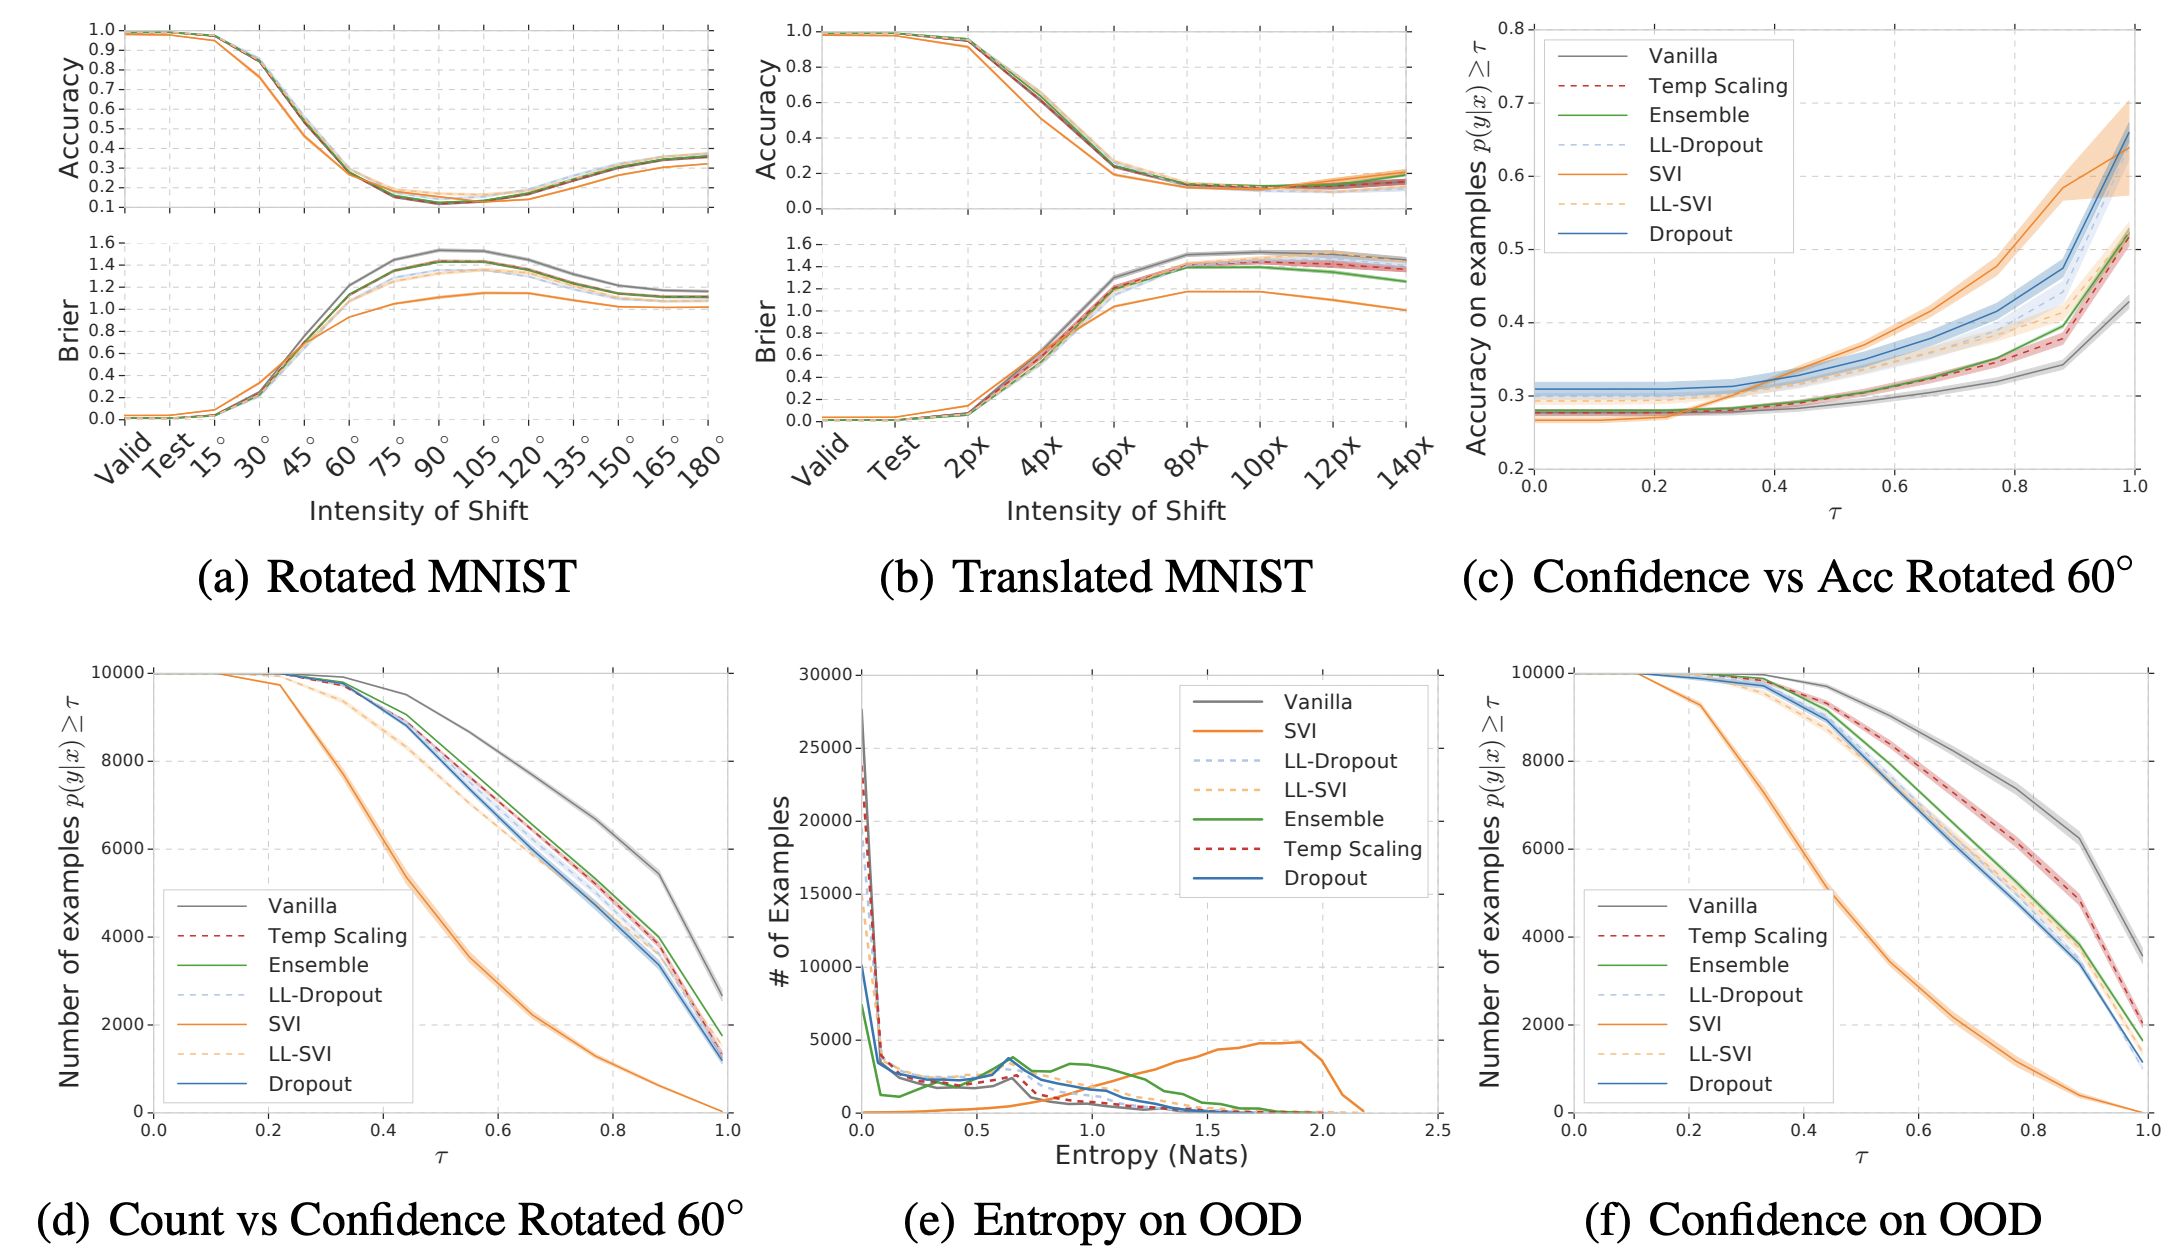
\includegraphics[scale=0.24]{images/figure1.png}
        \caption{(a) and (b): accuracy and Brier score as the data is increasingly shifted. Shaded regions represent standard error over 10 runs. %To understand the discrepancy between accuracy and Brier score, we explore
        The predictive distributions of each method by looking at the confidence of the predictions in (c) and (d).
        The entropy and confidence of each method on entirely OOD data in (e) and (f). SVI has lower accuracy on the validation and test splits, but it is significantly more robust to dataset shift %as evidenced by a lower Brier score, lower overall confidence (d) and higher predictive entropy under shift (c) and OOD data (e, f)
        }
        \label{fig:enter-label}
    \end{figure}
\end{frame}

\begin{frame}{Image Models: CIFAR-10 and ImageNet}
    \begin{figure}{}
        \centering
        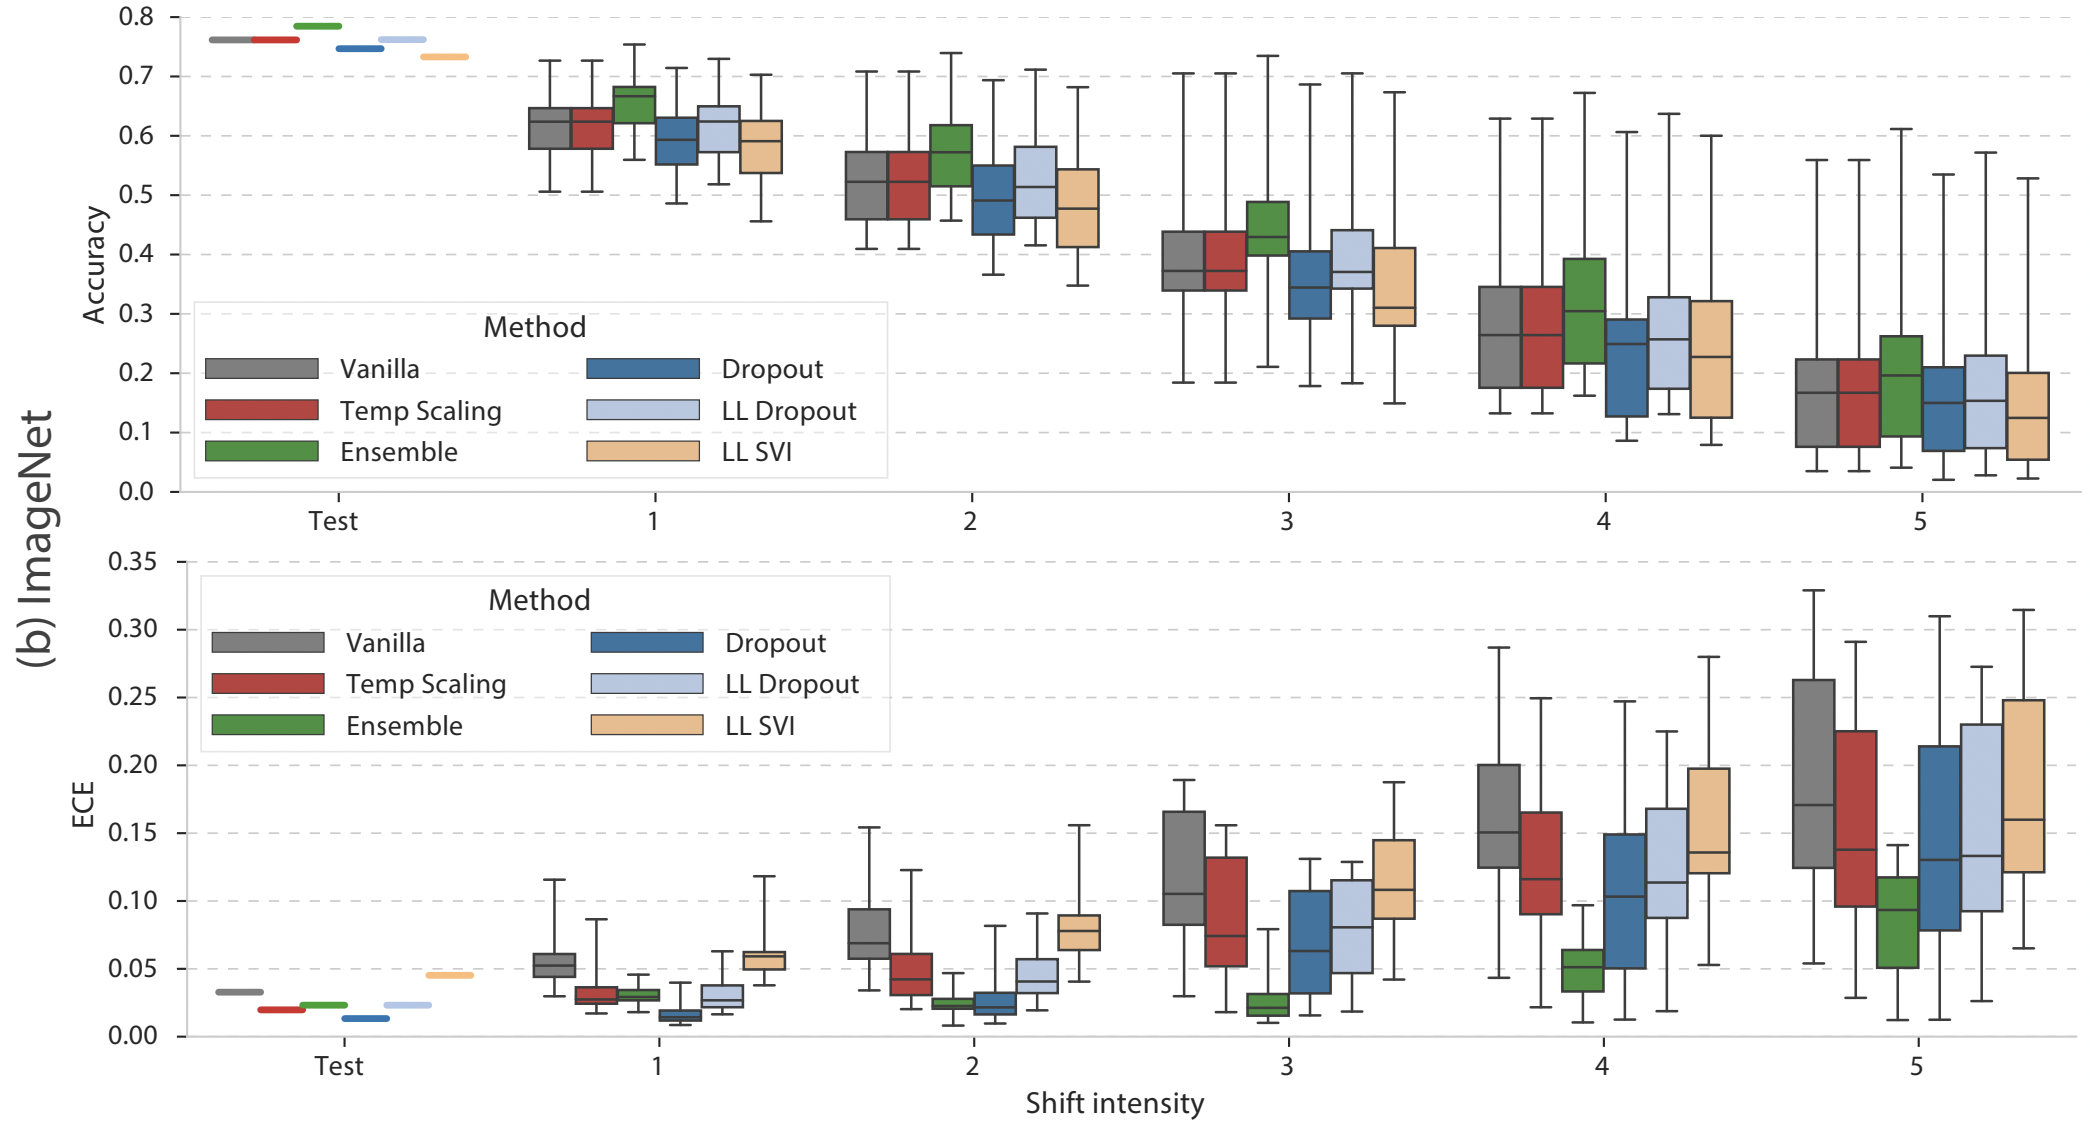
\includegraphics[scale=0.24]{images/imagenet.png}
        \caption{Calibration under distributional shift:  comparison of accuracy and ECE under
        all types of corruptions on ImageNet. For each method we show the mean on the test set and summarize the results on each intensity of shift with a box plot. Each box shows the quartiles summarizing the results across all (16) types of shift while the error bars indicate the min
        and max across different shift types.
        }
        \label{fig:enter-label}
    \end{figure}
\end{frame}

\begin{frame}{Image Models: CIFAR-10 and ImageNet}
    \begin{figure}{}
        \centering
        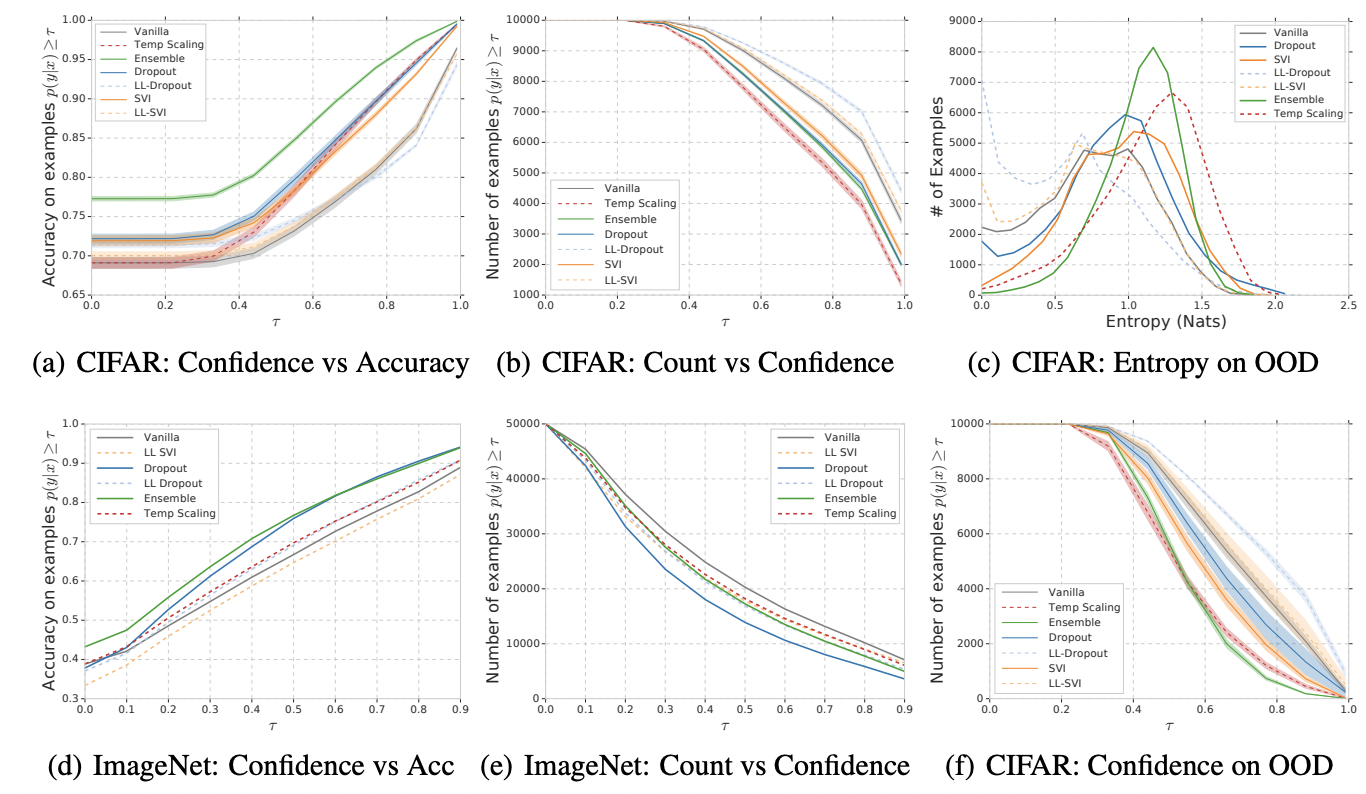
\includegraphics[scale=0.41]{images/figure3.png}
        \caption{left: accuracy as a function of confidence \\ middle: the number of examples greater than given confidence values for Gaussian blur of intensity 3\\ right: histogram of entropy and confidences from CIFAR-trained models on a completely different dataset (SVHN) (right column)}
        \label{fig:enter-label}
    \end{figure}
\end{frame}

\begin{frame}{Text Models}
    \begin{figure}{}
        \centering
        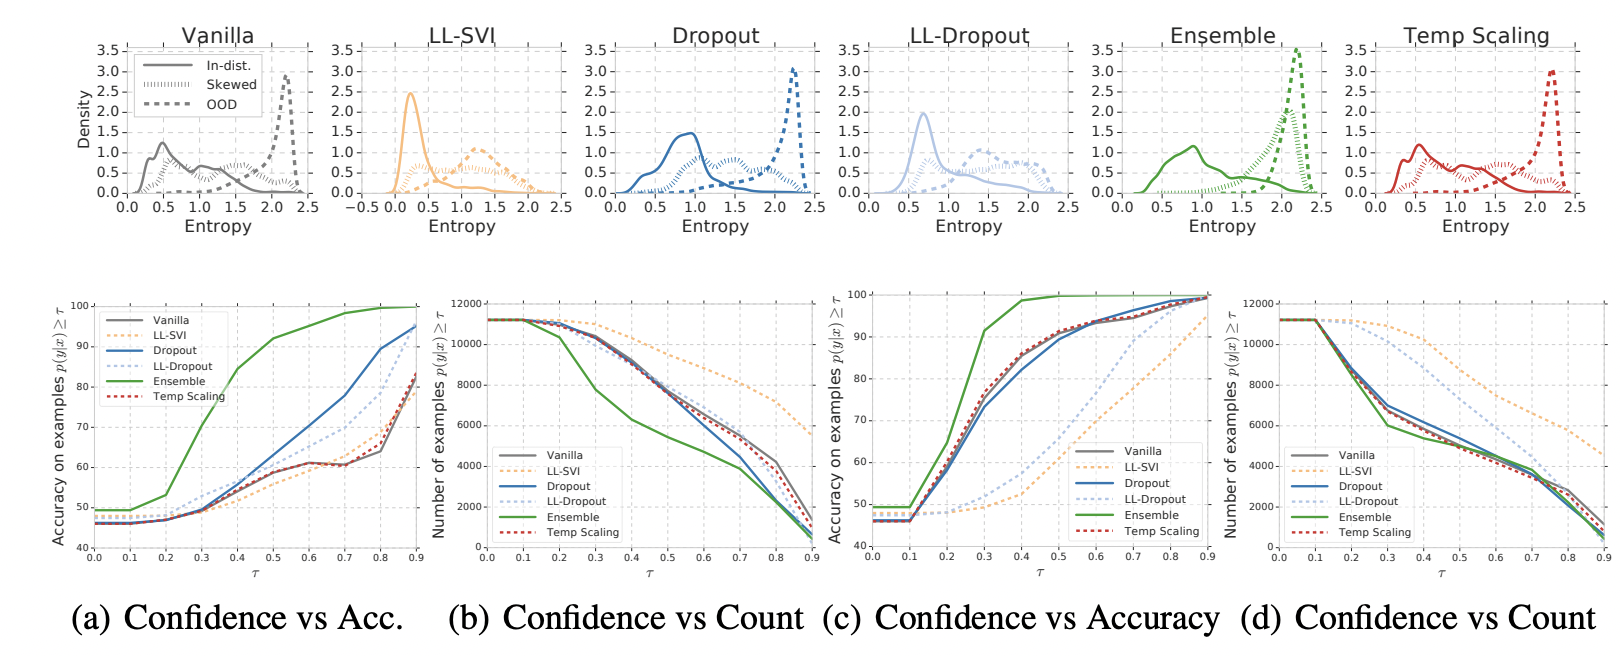
\includegraphics[scale=0.42]{images/figure4.png}
        \caption{Top row: Histograms of the entropy of the predictive distributions for in-distribution (solid lines), shifted (dotted lines), and completely different OOD (dashed lines) text examples. \\ Bottom row: Confidence score vs accuracy and count respectively when evaluated for in-distribution and
        in-distribution shift text examples (a,b), and in-distribution and OOD text examples (c,d)}
        \label{fig:enter-label}
    \end{figure}
\end{frame}


\begin{frame}{Ad-Click Model with Categorical Features}
    \begin{figure}{}
        \centering
        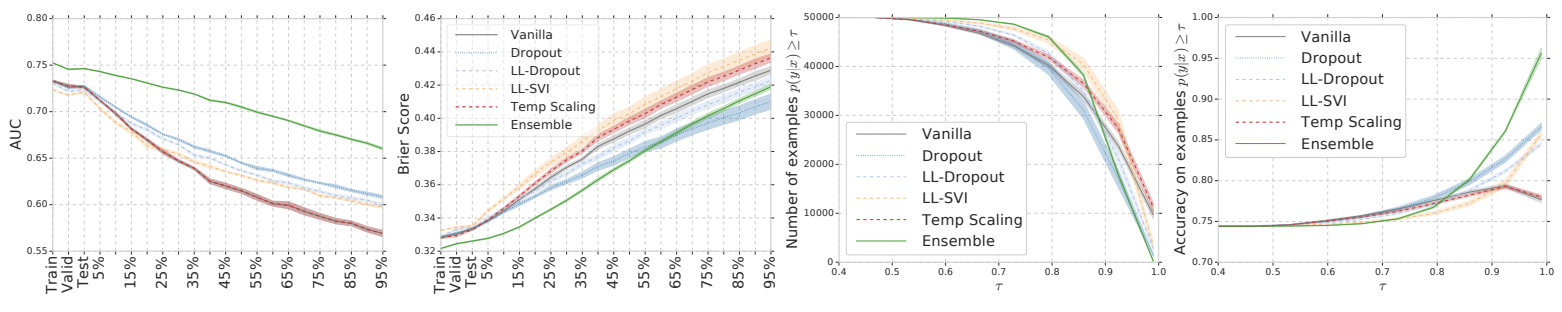
\includegraphics[scale=0.45]{images/figure5.png}
        \caption{Results on Criteo: The first two plots show degrading AUCs and Brier scores with increasing shift while the latter two depict the distribution of prediction confidences and their corresponding accuracies at 75 \% randomization of categorical features. SVI is excluded as it performed too poorly}
        \label{fig:enter-label}
    \end{figure}
\end{frame}



\begin{frame}{Takeaways and Recommendations}
    \begin{block}{Summary of Findings}
    % The paper presents a large-scale evaluation of methods for quantifying predictive uncertainty under dataset shift:
    \begin{itemize}
        \item Uncertainty quality degrades with increasing dataset shift.
        \item Calibration on i.i.d. test data does not ensure calibration under dataset shift.
        \item Temperature scaling on i.i.d. validation sets leads to better-calibrated uncertainty than baseline methods, especially with greater shifts.
        \item Last layer Dropout shows less uncertainty %on shifted/OOD datasets
        than Dropout.
        \item SVI is effective for small datasets but struggles with larger ones
        \item The relative ordering of methods is mostly consistent across exp-s % Exception: MNIST
        \item Deep ensembles generally outperform other methods%, especially on larger dataset shifts.
    \end{itemize}
    \end{block}
    \begin{block}{Recommendations for Future Work}
    It is recommended to explore more scalable and efficient methods for uncertainty quantification, especially under dataset shift. The benchmark set forth in this paper should inspire further research in this area.
    \end{block}
\end{frame}

\begin{frame}{Literature}
    \begin{enumerate}
        \item \textbf{Main article} \href{https://arxiv.org/pdf/1704.01168.pdf}
        {Can You Trust Your Model’s Uncertainty? Evaluating Predictive Uncertainty Under Dataset Shift}.
    \end{enumerate}
\end{frame}

\end{document}